% Chapter 3

\chapter{Experimental Design}

\label{Chapter4} % 

In this chapter we describe the different methods that were assessed for the task of predicting whether a user is interested in listening to music at time $t$ given their play history $h$. The methods, in order of gradually increasing sophistication, are as follows:

\begin{enumerate}
    \item Baseline model
	\item Bayesian Inference
	\item Binary Logistic Regression
	\item Linear SVM Classifier
	\item Non-Linear SVM Classifier
	\item Recurrent Neural Networks
\end{enumerate}

All methods, except for the Bayesian Inference method, require the data to be structured as a time-series. The Bayesian method adopts a different approach that requires the data to be aggregated into half-hourly buckets of a week.

The data preparation that was performed is described first in the next section, followed by an explanation each method, and the evaluaion criteria for assessing the methods.

\section{Data preparation}

\subsection{Data transformation}

The analysis was carried out in Python (via Jupyter notebooks) running on Ubuntu. The raw data consisted of timestamps of when a song was played and a user ID. These were loaded as-is into a SqlLite3 database in order to reduce the need to repeat data preparation steps.. The methods themselves utilized Scikit-learn for all models, save for the RNN model which used Tensorflow.

UserIDs were converted to integer (e.g. 'User0005' became '5') and a period lookup table was created at n minute intervals, to which all timestamps in our main dataset could be mapped to. n was chosen to be 30 although it is possible to re-run the analysis for other levels of granularity.


More significantly the data, which contained entries for the times at which each user listened to music, was supplemented with all the times they did \emph{not} listen to music, between their date of their first and last play.  This was required in order to generate a sequence of play and non-play events. It was noted however that in cases where a user stops listening to music for a long period, then listens to it sporadically, we would get an even greater imbalance of data (see later).

\subsection{Time-series fetures}

The approach to feature selection for this research was to devise an initial of features based on the preliminary analysis, and use that list across all models.

The time series features that were derived from the raw data were time-lags: $t, t-1, t-2, t-3, t-4, t-5,  t-12hrs, t-23.5hrs, t-24hrs, t-24.5hrs, t-1wk, t-2wks, t-3wks, t-4wks$ where t is the event being predicted. 

$t-1$ to $t-5$ represent user activity in the previous 2.5 hours. The remaining time-lags were chosen to represent half-day, daily, and weekly cycles, with additional empahsis around the -24 hour mark due to the daily patterns observed in the preliminary analsysis (see next chapter).  

In addition a few non-time lag features were selected. One of which was the number of hours away from 5pm in either direction (so a timestamp at 4pm and 6pm would both equal 1), based on the observations in the preliminary analysis of 5pm being a peak hour.
The others were binary features representing the day of the week (isMon, isTue etc.). Again these were based on the patterns observed in the preliminary analysis.

To improve the speed and quality of our models, rows where all time-lags indicated a non-play were removed from the dataset. Only 0.62\% of such cases were found to be a play-event at time $t$.

\section{Validation and Test dataset selection}

Our working dataset was a subset of the full 1000 user dataset, and comprised of 4,217,228 rows of training data across 97 users. Of this a random sample of 100,000 rows was taken on which 5-fold cross-validation. 

Due to the time it takes for training cross validation was not performed on the RNN model, instead 10 randomly selected users were held back from the main training dataset and a random sample of 10,000 rows were taken from each user.

\subsubsection{Data Imbalance}

Data imbalance is when the training data is when one or more of the classes is under-represented in the dataset. Of the 4,217,228 rows in our data set, 361,081 (8.6\%) were play events and 91.4\% were non-play events.  

This could lead to models that achieve a high accuracy score by following either or both of the following two heuristcs:
* Predict non-event for everything
* Predict $t$ will be the same as $t-1$

There are several methods for dealing with data imbalance \parencite{Brownlee} including restricting input data, having a weighted loss function, and using recall as an evaluation measure.

In this research class weights were employed to automatically adjust weights inversely proportional to class frequencies in the input data $n_samples / (n_classes * np.bincount(y))$.

This would have the impact of encourgaing the model to predict play events more frequently. However our goal is to encourage the model to predict play events, while minimizing the number of false postivies on the predicitions (i.e. we attach less cost to false-positives for non-event prediction). Encouraging this sort of behaviour requires not only class weighting, but also sample weighting to give a higher penalty to false positives for play-predictions. This strategyh was also employed in the models as shown in the following Python snippet (1 represents a Play event):

$$sampleWeights =  1+(y[:] == 1) * (x[:,1] ==0)$$

\section{Methods}

\subsection{Baseline Model}

Our baseline model will be to assume $t = t-1$, that is to say a person will listen to music at period $t$ if, and only if, they listened to music in the period immediately priod. As music listening events tend to be clustered (people listen to music in batches) the accuracy of the baseline model is expected to be fairly high. However it will not be able to predict the first play of a listening session, or where the listening session duration lasts no longer than a single periodm, which in the experiments is defined as a 30 minute period.

\subsection{Bayesian Inference}

We employ a simple Bayesian Inference approach by utilizing the Beta-Binomial model. The Beta-Binomial model is built upon the weekly patterns observed in the preliminary analysis. Conceptually it seeks to build up a users personalized weekly listening profile as observations come in, using a Beta-Binomial probability distribution, with the priors based on the population as a whole. We then assess how effective this profile is at predicting listening events for that user.

Prior probabilities were calculated or each half-hourly period in a week (24*2*7=336 timeslots). Fig \ref{fig10b} shows the calculations for the first 2.5 hours of a Sunday (d-hour-hh format). 

The liklihood function which represents the probability of a user listening to music was defined as a binomial distribution, where $k$ is the number of plays in a given period, $n$ is the sum of plays and non-plays, and $\theta$ is the unknown probability parameter for the binomial distribution.

$${n \choose k}\,p^{k}(1-p)^{n-k}$$

As the Beta distribution is a conjugate prior to the Binomial the model can be reduced to: $Beta(\alpha+P, \beta+Q)$ where P is the count of plays and Q is the count of non-plays.

Our parameters for the beta distribution, $\alpha$ and $\beta$, are derived from the training set, with an estimate of the mean for each half-hourly time period as shown in fig \ref{fig10b}. 

\begin{figure}[h!]
	\centering
	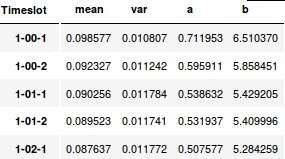
\includegraphics[width=4cm, keepaspectratio,]{fig010b.jpg}
	\caption{}
	\label{fig10b}
\end{figure} 

We first calculate the probability of a play (total plays in period / count of plays and non-plays) per user, then take the mean and variance across users. $a$ and $b$ are then determined as:
$a = (\frac{(1- \mu)}{\sigma} - \frac{1}{\mu}) \mu^2$
and
$\beta=\alpha\left(\frac{1}{\mu}-1\right)$.

Finally we convert the probabilites into a binary outcome by optimizing for a threshold $\lambda$ at which we predict a play event.

\subsection{Binary Logistic Regression}

This method (and the subsequent methods) adopts a more classicial time-series approach to the prediction problem by constructing a dataset as a sequence of play events at time t $Y_t = 1$ and non-play events $T_t = 0$ with $t$ representing a time period of a fixed interval, which for our research will be 30 minute chunks. We seek to calculate the probability of an event in the current time period $t$, given the history of events: $p(Y_t =1 \mid Y_h)$, for each individual user together with additional non-time-series features (see . 

Our binary logistic model is therefore defined as:
$$p(Y_t = 1|Y_h) = \sigma(w^Tx + b)$$
$$p(Y_t = 1|Y_h) = 1 - p(Y_t = 1|Y_h)$$

with $\sigma$ being the sigmoid function defined as:
$$\sigma(x)=\frac{e^x}{1+e^x}$$

Determining the optimal weights and constant can be determined by maximization of the log-liklihood or the minimization of the negative log-liklihood \parencite{NegLog}. The latter is given as:

$$Csum^n_{i=1}log(exp(-y_i(X^T_iw+b))+1)$$

for class $C = 1$.

In addition we will be comparing results with and withour the L2 regularizer term:
 $ + 1/2w^Tw$

Regularization is technique for encouraging the model to converge on a smaller set of strong features rather than a wide set of weak features and is imporant in helping us determine which time-lags and additional features are important and which are not.

\subsection{Linear SVM Classifier}

SVM models seek to determine a separation plane between classes based on the support vectors, the data points closes to the decision boundary.

A linear SVM regression model performs this through the Epsilon Intesive loss function \parencite{Vapnik}. The objective becomes to \textit{minimize:}

$$max(0,\left\| (y_i - w_i x_i - b) - \epsilon \right\|)$$

In other words we ignore cost functions that are within a certain margin  $\epsilon$. In our case this may be of importance in cases where the probability of user listening to music is close to the decision boundary, which may be the case for the very first song played at the start of a session.

\subsection{Non-Linear SVM Classifier}

Here we extend a regression model to include a Gaussian RBF kernel. A Gaussian kernel is a popular method for modeling non-linear decision boundaries, so for example if the decision to play music is based on some non-linear combination of day of the week, time of the day, and time since last play. Our model becomes:

$$p(E=1)=b+\sum^N_{i=1}w_iRBF(x,x_i)$$

where the RBF kernel is defined as:

$$K(\mathbf {x} ,\mathbf {x'} )=\exp \left(-{\frac {\|\mathbf {x} -\mathbf {x'} \|^{2}}{2\sigma ^{2}}}\right)$$

Note that our actual implementation in Tensorflow makes use of the more computationally efficient algorithm as defined by McClure \parencite{TFCookbook}. This restated method has a parameter $\gamma$ that takes the place of $2\sigma^2$ and which requires tuning.

Mini-batching was also performed with a batch size of 2000 and 5 iterations of the dataset, as it was found that rows of more than 5000 caused memory errors, and iterations beyond 5 showed minimal or no decrease in loss).

\subsection{Recurrent Neural Networks}

Recurrent nets are a type of artificial neural network designed to recognize patterns in sequences of data, such as text, genomes, handwriting, the spoken word, or numerical times series data emanating from sensors, stock markets and government agencies. Whilst a traditional Feed-Forward network \parencite{MLP} has input nodes, hidden layers, and an output layer, with data flowing in one direction only, RNNs allow for the hidden state from one timestep of the neural net to be an input into the next (see fig. \ref{RNN}).

\begin{figure}[h!]
	\centering
	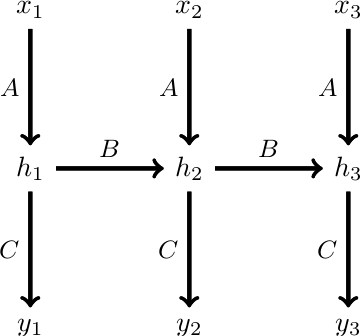
\includegraphics[width=3cm, keepaspectratio,]{fig007.jpg}
	\caption{RNN with 3 timesteps}
	\label{RNN}
\end{figure} 

RNN models can employ different methods the propogration of the hidden state over time. One such well known method is Long Short-Term memory (LSTM) \parencite{Olah}. Here the hidden state is the product of a further four layers that interact in a way as to learn what information to retain and what information to throw away. 

\begin{figure}[h!]
	\centering
	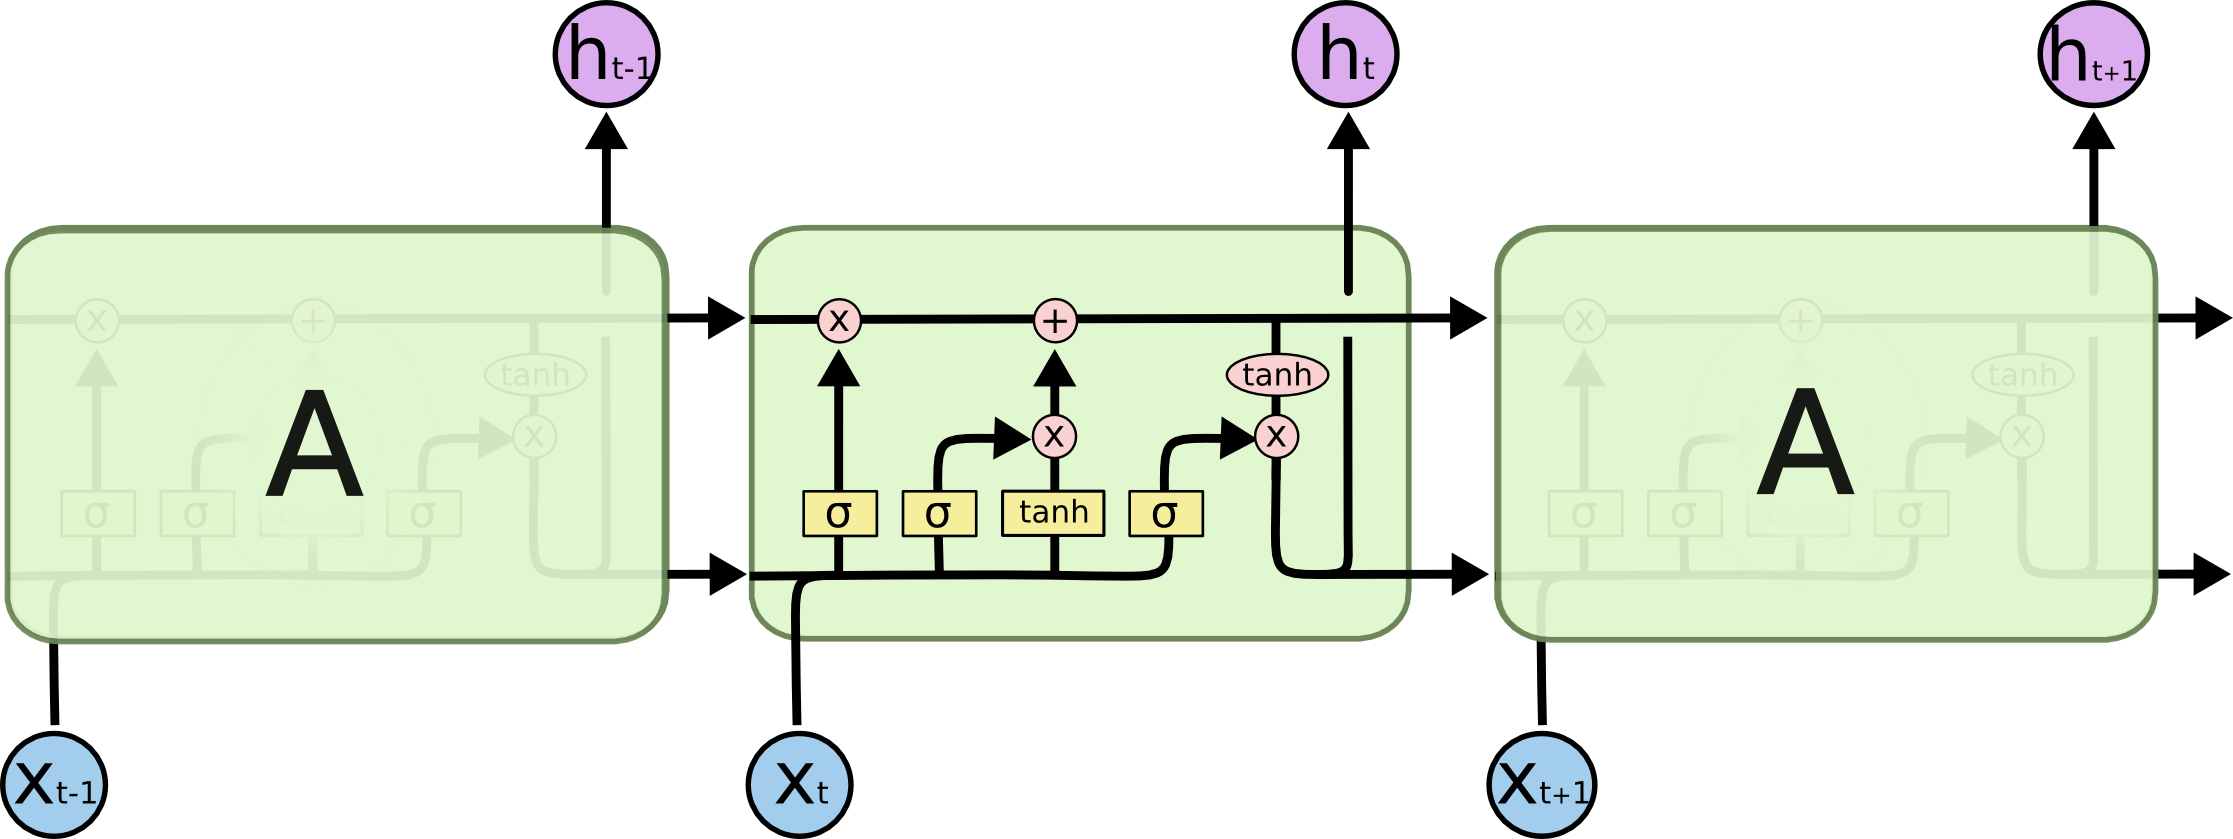
\includegraphics[width=5cm, keepaspectratio,]{fig008.png}
	\caption{LSTM}
	\label{fig:fig8}
\end{figure} 


We could therefore provide the model with a sequence of historical data at times $t-1 .. t-n$ where $n >1)$ which would be fed into the RNN as separate time steps in forward temporal order. The hidden state would propogate information from $t_n$ forward at each time step, until it was used to predict the outcoem a time $t$.

Practically speaking this mean feeding in the data with input shape (batch rows, time-steps, features). Some points of interest to fellow researchers are:

\begin{enumerate}
	\item The features dimension here does not need to contain all time-lags as we do in our other time-series models. However it must contain t-1. In this research we experiment with both t1 only and all our timelag features in this research.
		
	\item The time-steps dimension is where the features list in previous time steps will be stored. These are then 'unrolled' within Tensorflow and fed into the LSTM. In this research we experiment with different lengths of time-steps.

	\item When the data is unrolled, time step $t$ for all rows in the batche are processed together as one block, before moving onto the next time-step.

	\item Constructing the 3-d shape often requires building them up in slices. A significant speed up was observed in Python when using a pre-allocated array vs. appending to it.
\end{enumerate}

\section{Evaluation critera}

Deciding on an approporiate evaluation measure requires careful consideration to the costs attached to different predictions. In our case we assign a lower cost to predicting a non-play event, and being wrong, than predicting a play-event and being right (as the cost of suggesting music when the user is likely not interested is higher than not playing music when they likely not interested). 

We also wish to rate models higher if they manage to predict the first play of a listening session, as this is seen be harder than simply predicting a play event, when the last n events were also a play event.

With these in mind a number of possible evaluation criteria were looked at. The most-straight forward of which was \textit{accuracy}. This computes the count of correct predictions as a fraction of the total number of predictions. While this is an intuitive measure, it would not distinguish between models that had a high accuracy on the play-events vs. a high accuracy on non-play events. 

To do this we look at precision. Precision (P) is defined as the number of true positives over the number of true positives plus the number of false positives. A positive in this case is a play-event so our precision equation becomes:

$$Precision = \frac{Correct Play Predictions}{Total Play Predictions}$$. 

This will be measuring our models on how many of their play event guesses were correct which takes care of one of our considerations outlined above. However it does not distinguish between models that predict a play event only when the previos event was a play (a 'safe bet' and so a high precision score) vs. models that predict correctly in cases where the previous event was not a play and are threfore harder to get right. We turn to another measure to aid with this: recall.

Recall is defined as the number of true positives over the number of true positives plus the number of false negatives. A false negative is where a model predicts a non-event, when in fact there was an event. For example if we predicted 100 plays correctly but there were in fact 110 plays in the dataset, then recall would be 100/(100 + 10)= 91%.

$$Recall = \frac{CorrectPlayPredictions}{TotalPlayPrectionsInDataset}$$

Precision and recall in combination was therefore our chosen evaluation method. In addition tests were carried out examine how well the models performed on predicting the first play event in a series.



\section{Summary}

We have described how our data was transformed to make it useful for our experiments. In particular how we had to convert our list of play events into a list of play and non-play events for every period. By doing this we are faced with an imbalance of data as non-play events make up ~91\% of the data and so we employ a weighting strategy to counteract this.

We then described the methods we will be utilizing in our experiments, consisting of a Baseline model which is simply to assume $t =t-1$, a Bayesian model which build up a weekly profile of listening habits for each user, Logistic and SVM models that apply classical machine learning time-series prediction techniques to our problem, and finally a deep learning model in the form of an RNN-LSTM where we seek to utlize the capabilities for it to learn temporal patterns through a hidden memory state.

Finally we looked at different ways for measuring the success of our problem, with precision and recall being the preferred choice.

In the next chapter we shall present the results of our experiements and a discussion of what this tells us about learning user-level temporal patterns and performing event prediction.